% Copyright (C) 2007 Technical University of Liberec.  All rights reserved.
%
% Please make a following reference to Flow123d on your project site if you use the program for any purpose,
% especially for academic research:
% Flow123d, Research Centre: Advanced Remedial Technologies, Technical University of Liberec, Czech Republic
%
% This program is free software; you can redistribute it and/or modify it under the terms
% of the GNU General Public License version 3 as published by the Free Software Foundation.
%
% This program is distributed in the hope that it will be useful, but WITHOUT ANY WARRANTY;
% without even the implied warranty of MERCHANTABILITY or FITNESS FOR A PARTICULAR PURPOSE.
% See the GNU General Public License for more details.
%
% You should have received a copy of the GNU General Public License along with this program; if not,
% write to the Free Software Foundation, Inc., 59 Temple Place - Suite 330, Boston, MA 021110-1307, USA.
%
%%%%%%%%%%%%%%%%%%%%%%%%%%%%%%%%%%%%%%%%%%%%%%%%%%%%%%%%%%%%%%%%%%
%
% use PDFLatex to compile this
%

\documentclass[a4paper]{article}

% our own flow_doc.sty
%\usepackage{flow_doc}

%\usepackage{rotating}
%\usepackage{pdflscape}

\usepackage{amssymb, amsmath, amsthm}
\newtheorem{theorem}{Theorem}


\usepackage{array}
\usepackage{longtable}
%\usepackage[usenames,dvipsnames]{color}   %colors
%\usepackage{colortbl}   %colorful tables
\usepackage{tabularx}
\usepackage{graphicx} %[dvips]
% it is note used \usepackage{cooltooltips}

%these two can be found in caption package
%\usepackage{caption}
%\usepackage{subcaption}

\usepackage[numbers]{natbib}

%\usepackage{fancyvrb}   % extended verbatim environments (for examples of IO files)

%\usepackage{multicol}
\usepackage{etoolbox}


%%%%%%%%%%%%%%%%%%%%%%%%%%%%%%%%%%%%%%%%%%%%%%%%%%%%%%%%%%%%%%%%%%%%%%%%%%%%
% macro for units 
\def\UNIT#1#2{\ifstrempty{#2}{}{%
\ifstrequal{#2}{1}{\mathrm{#1}}{\mathrm{#1}^{#2}}%
}}
\def\units#1#2#3{\ifstrempty{#1#2#3}{$[-]$}{$[ \UNIT{kg}{#1}\UNIT{m}{#2}\UNIT{s}{#3} ]$}}       %with brackets
\def\unitss#1#2#3{\ifstrempty{#1#2#3}{$-$}{$ \UNIT{kg}{#1}\UNIT{m}{#2}\UNIT{s}{#3} $}}  %without brackets


\newcommand{\vari}[1]{{\it #1}}
\newcommand{\ditem}[2]{\item[\vari{#1} {\tt #2}]}
\newenvironment{fileformat}{\tt\begin{flushleft}}{\end{flushleft}}

%%%%%%%%%%%%%%%%%%%% specific math macros
\def\prtl{\partial}
\def\vc#1{\mathbf{\boldsymbol{#1}}}     % vector
\def\tn#1{{\mathbb{#1}}}    % tensor
\def\abs#1{\lvert#1\rvert}
\def\Abs#1{\bigl\lvert#1\bigr\rvert}
\def\div{{\rm div}}
\def\Lapl{\Delta}
\def\grad{\nabla}
\def\Real{{\mathbf R}}
\def\d {\,{\rm d}}
\def\Natural{\mathbf N}
\def\norm#1{\|#1\|}
%% ini_table members
%%%%%%%%%%%%%%%%%%%% specific math macros


%%%%%%%%%%%%%%%%%%%%%%%%%%%%%%%%%%%%%%%%%%%%%%%%%%%%%%%%%%%%%%%%%%%%%%%%%%%%%%%%%%%%%%%%%%%%% BEGIN DOCUMENT
%% set specific page layout
%\addtolength{\textwidth}{2cm}
%\addtolength{\hoffset}{-1.5cm}
%\addtolength{\textheight}{4cm}
%\addtolength{\voffset}{-2.5cm}
\begin{document}

\section{Quick start}

Flow123D is a software for simulation of water flow, reactionary solute transport and heat transfer in a heterogeneous 
porous and fractured medium. In particular it is suited for simulation of underground processes in a granite rock massive.
The program is able to describe explicitly processes in 3D medium, 2D fractures, and 1D channels and exchange between 
domains of different dimensions. The computational mesh is therefore a collection of tetrahedra, triangles and line segments.

The water flow model assumes a saturated medium described by the Darcy law. For discretization, we use lumped mixed-hybrid finite element method.
We support both steady and unsteady water flow. The water flow model can be sequentially coupled with two different models for a solute transport or with a heat transfer model.

The first solute transport model can deal only with pure advection of several substances without any diffusion-dispersion term. It uses 
explicit Euler method for time discretization and finite volume method for space discretization and operator splitting method to 
couple with various processes described by the reaction term. The reaction term can treat any meaningful combination of the dual porosity, adsorptions, decays and linear reactions.
Alternatively, one can use interface to the experimental SEMCHEM package for more complex geochemistry.

The second solute transport model describes general advection with hydrodynamic dispersion for several substances. It uses implicit Euler method for time discretization and discontinuous Galerkin method of
the first, second or third order for the discretization in space. Currently there is no support for reaction term, the operator splitting approach (although it is not suited for implicit time schemes) 
is planned for the next version.

The heat transfer model assumes equilibrium between temperature of the rock and the fluid phase. It uses the same numerical scheme as the second transport model.

The program support output of all input and many output fields into two file formats. You can use file format of GMSH mesh generator and post-processor 
or you can use output into widely supported VTK format. In particular we recommend Paraview software for visualization and post-processing of the VTK data.

The program is implemented in C/C++ using essentially PETSC library for linear algebra. All models can run in parallel using MPI environment, however, 
the scalability of the whole program is limited due to serial mesh and serial outputs.


The program is distributed under GNU GPL v. 3 license and is available on the project web page:
\verb'http://flow123d.github.io'

with sources on the GitHub:
\verb'https://github.com/flow123d/flow123d'.


\section{Mathematical models \\of physical reality}
\label{PhysicalModels}

Flow123d provides models for Darcy flow in porous media as well as for the transport and reactions of solutes. In this section, we describe 
mathematical formulations of these models together with physical meaning and units of all involved quantities. In the first section we present 
basic notation and assumptions about computational domains and meshes that combine different dimensions. In the next section we
derive approximation of thin fractures by lower dimensional interfaces for a general transport process. Latter sections describe details for models of particular
physical processes.

\subsection{Meshes of mixed dimension}
Common and unique feature of all models in Flow123d is the support of
domains with mixed dimension. 
Let $\Omega_{3} \subset \Real^3$ be an open set representing continuous approximation of porous and fractured medium.
Similarly, we consider a 2D manifold $\Omega_2\subset\overline\Omega_3$, representing 2D fractures and a 1D manifold $\Omega_1\subset \overline\Omega_2$ of 1D channels or preferential paths (see Fig \ref{fig:multi-dim}).
We assume that $\Omega_2$ and $\Omega_1$ are polytopic (i.e. polygonal and piecewise linear, respectively).
For every dimension $d=1,2,3$, we introduce a triangulation $\mathcal{T}_{d}$ of the open set $\Omega_d$
that consists of finite elements $T_{d}^{i},$\ $i = 1,\dots,N_{E}^{d}$.
The elements are simplices, i.e. lines, triangles and tetrahedra, respectively.

\begin{figure}[h]
\centering
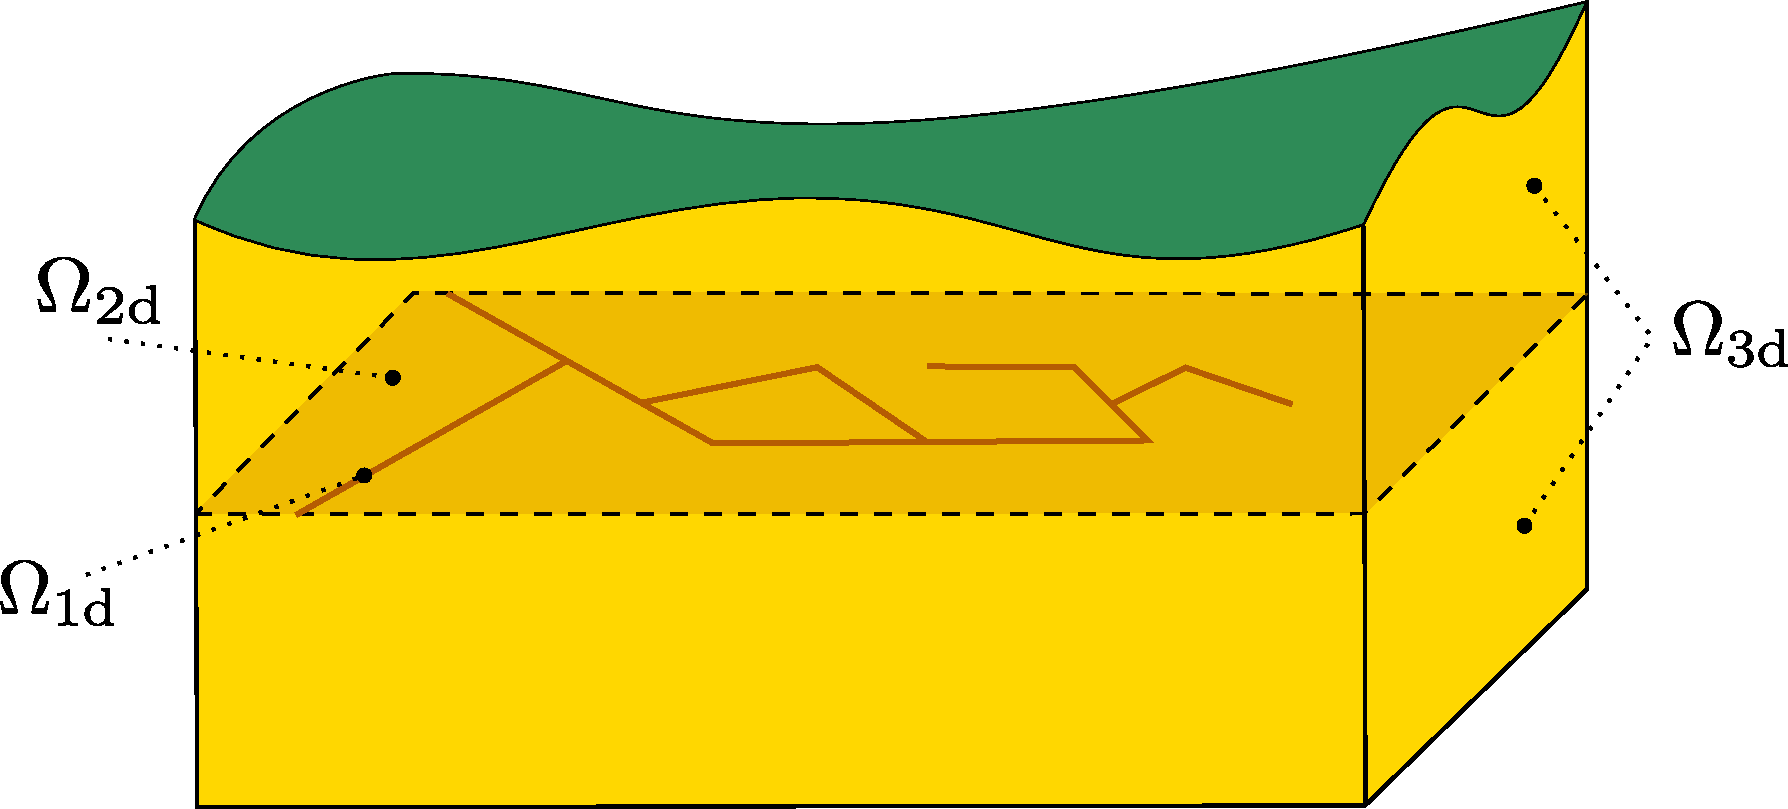
\includegraphics[width=10cm]{figures/ground_fractures}
\caption{
    \label{fig:multi-dim}
    Scheme of a problem with domains of multiple dimensions.
}
\end{figure}

Present numerical methods require meshes satisfying the compatibility conditions
\begin{equation}
        T_{d-1}^i \cap T_d \subset \mathcal{F}_d,   \qquad \text{where } \mathcal{F}_d = \bigcup_{k} \partial T_{d}^{k}
\end{equation}
and
\begin{equation}
        T_{d-1}^i \cap \mathcal{F}_d    \text{ is either $T_{d-1}^i$ or $\emptyset$}    
\end{equation}
for every $i\in\{1,\dots, N_{E}^{d-1}\}$, $j\in\{1,\dots,N_{E}^{d}\}$,  and $d=2,3$. That is, the $(d-1)$-dimensional elements are either between $d$-dimensional elements and
match their sides or they poke out of $\Omega_d$. 

\subsection{Advection-diffusion processes on fractures}
\label{sc:ad_on_fractures}
In this section, we shall derive a model for a general advection-diffusion process in a domain of mixed dimensions using
simple approximations inspired by the paper \citet{martin_modeling_2005}. Let us consider a fracture as a strip domain 
\[
 \Omega_f \subset [0,\delta] \times \Real^{d-1}
\]
for $d=2$ or $d=3$ and surrounding continuum domains
\[
 \Omega_1 \subset (-\infty,0)\times \Real^{d-1},
 \Omega_2 \subset (\delta,\infty)\times \Real^{d-1}.
\]
Further, we denote by $\gamma_i$, $i=1,2$ the fracture faces common with domains $\Omega_1$ and $\Omega_2$ respectively.
By $x$, $\vc y$ we denote normal and tangential coordinate of a point in $\Omega_f$. 
We consider the normal vector  $\vc n=\vc n_1=-\vc n_2=(1,0,0)^\top$.
An advection-diffusion process is given by equations:
\begin{align}
  \label{eq:fr:continuity}
  \prtl_t w_i + \div \vc j_i &= f_i&&  \text{on } \Omega_i,\ i=1,2,f,\\
  \label{eq:fr:flux}
  \vc j_i &= - \tn A_i\grad u_i + \vc b_i w_i&& \text{on } \Omega_i,\ i=1,2,f,\\
  \label{eq:fr:Dirichlet}
  u_i &= u_f&& \text{on } \gamma_i,\ i=1,2,\\
  \label{eq:fr:Neumann}
  \vc j_i \cdot \vc n &= \vc j_f \cdot \vc n&& \text{on } \gamma_i,\ i=1,2,
\end{align}
where $w_i=w_i(u_i)$ is the conservative quantity and $u_i$ is the principal unknown, $\vc j_i$ is the flux of $w_i$, $f_i$ is the source term,
$\tn A_i$ is the diffusivity tensor and $\vc b_i$ is the velocity field. We assume that the tensor $\tn A_f$ is symmetric positive definite 
with one eigenvector in the direction $\vc n$. Consequently the tensor has the form:
\[
 A_f = \begin{pmatrix} 
            a_n & 0  \\
            0 & \tn A_t
       \end{pmatrix}
\]
Furthermore, we assume that $\tn A_f(x, \vc y)=\tn A_f(\vc y)$ is constant in the normal direction.

Our next aim is to integrate equations on the fracture $\Omega_f$ in the normal direction 
and obtain their approximations on the surface $\gamma=\Omega_f \cap \{x=\delta/2\}$ running through the middle of the fracture. 
For the sake of clarity, we will not write subscript $f$ for quantities on the fracture. 
To make the following procedure mathematicaly correct we have to assume that functions
$\prtl_x w$, $\prtl_x \grad_{\vc y} u$, $\prtl_x \vc b_{\vc y}$ are continuous and bounded on $\Omega_f$. Here and later on 
$\vc b_x=(\vc b \cdot \vc n)\, \vc n$ is the normal part of the velocity field and $\vc b_{\vc y} = \vc b - \vc b_x$ is the tangential part.
The same notation will be used for normal and tangential part of the field $\vc q$.

We integrate \eqref{eq:fr:continuity} over the fracture opening $[0,\delta]$ and use approximations to get
\begin{equation}
    \label{eq:fracture_continuity}
   \prtl_t (\delta W) - \vc j_2 \cdot \vc n_2 - \vc j_1 \cdot \vc n_1 + \div \vc J = \delta F,
\end{equation}
where for the first term, we have used mean value theorem, first order Taylor expansion, 
and boundedness of $\prtl_x w$ to obtain approximation:
\[
    \int_0^\delta w(x,\vc y) \d x=\delta w(\xi_{\vc y}, \vc y) = \delta W(\vc y) + O(\delta^2\abs{\prtl_x w}),
\]
where
\[
    W(\vc y)=w(\delta / 2,\vc y)=w(u(\delta/2,\vc y))=w(U(\vc y)).
\]
Next two terms in \eqref{eq:fracture_continuity} come from the exact integration 
of the divergence of the normal flux $\vc j_x$.
Integration of the divergence of the tangential flux $\vc j_{\vc y}$ gives the fourth term, where we introduced
\[
\vc J(\vc y) = \int_0^\delta \vc j_{\vc y}(x, \vc y) \d x.
\]
In fact, this flux on $\gamma$ is scalar for the case $d=2$. Finally, we integrate the right-hand side to get 
\[
    \int_0^\delta f(x,\vc y) \d x = \delta F(\vc y) + O(\delta^2\abs{\prtl_x f}),\quad F(\vc y)=f(\delta/2,\vc y). 
\]


Due to the particular form of the tensor $\tn A_f$, we can separately integrate tangential and normal
part of the flux given by \eqref{eq:fr:flux}. Integrating the tangential part and using approximations
\[
    \int_0^\delta  \grad_{\vc y} u(x, \vc y) \d x = \delta \grad_{\vc y} u (\xi_{\vc y}, \vc y) 
    = \delta \grad_{\vc y} U( \vc y) + O\big( \delta^2 \abs{\prtl_x\grad_{\vc y} u} \big) 
\]
and
\[
 \int_0^\delta \big(\vc b_{\vc y} w\big)(x, \vc y) \d x 
  = \delta \vc B(\vc y) W(\vc y) + O\big(\delta^2 \abs{\prtl_x(\vc b_{\vc y} w)} \big)
\]
where
\[
  \vc B(\vc y) = \vc b_{\vc y}(\delta/2, \vc y),
\]
we obtain
\begin{equation}
    \label{eq:fracture_darcy}
   \vc J = -\tn A_t \delta \grad_{\vc y} U + \delta \vc B W + O\big(\delta^2(\abs{\prtl_x\grad_{\vc y} u}+\abs{\prtl_x(\vc b_{\vc y} w)})\big).
\end{equation}


So far, we have derived equations for the state quantities $U$ and $\vc J$ on the fracture manifold $\gamma$. In order to
get a well possed problem, we have to prescribe two conditions for boundaries $\gamma_i$, $i=1,2$. To this end, we
perform integration of the normal flux $\vc j_x$, given by \eqref{eq:fr:flux}, separately for the left and right half of the fracture.
Similarly as before we use approximations
\[
 \int_0^{\delta/2} \vc j_x \d x = (\vc j_1 \cdot \vc n_1)\frac{\delta}{2} + O(\delta^2 \abs{\prtl_x \vc j_x})
\]
and 
\[
 \int_0^{\delta/2} \vc b_x w \d x = (\vc b_1 \cdot \vc n_1)\tilde{w}_1\frac{\delta}{2} + O(\delta^2 \abs{\prtl_x \vc b_x}\abs{w} + \delta^2\abs{\vc b_x}\abs{\prtl_x w})
\]
and their counter parts on the interval $(\delta/2, \delta)$ to get
\begin{align}
    \label{eq:fracture_normal_1}
     \vc j_1 \cdot \vc n_1 &= -\frac{2a_n}{\delta} (U - u_1) + \vc b_1\cdot \vc n_1 \tilde{w}_1\\
    \label{eq:fracture_normal_2}
    \vc j_2 \cdot \vc n_2 &= -\frac{2a_n}{\delta} (U - u_2) + \vc b_2\cdot \vc n_2 \tilde{w}_2
\end{align}
where $\tilde w_i$ can be any convex combination of $w_i$ and $W$. Equations \eqref{eq:fracture_normal_1}  
and \eqref{eq:fracture_normal_2} have meaning of a semi-discretized flux from domains $\Omega_i$ into fracture.
In order to get a stable numerical scheme, we introduce a kind of upwind already on this level using a different convex 
combination for each flow direction:
\begin{align}
   \notag 
   \vc j_i \cdot \vc n_i
       = &-\sigma_i (U - u_i)      \\ 
   \notag
      &+ \big[\vc b_i\cdot \vc n_i\big]^{+} \big(\xi w_i + (1-\xi) W\big)       \\
      \label{eq:fracture_normal}
      &+ \big[\vc b_i\cdot \vc n_i\big]^{-} \big((1-\xi) w_i + \xi W\big), \qquad i=1,2
\end{align}
where $\sigma_i = \frac{2a_n}{\delta}$ is the transition coefficient and the parameter $\xi\in [\frac12, 1]$ can be used to interpolate
between upwind ($\xi = 1$) and central difference ($\xi=\frac12$) scheme. Equations \eqref{eq:fracture_continuity}, \eqref{eq:fracture_darcy}, and
\eqref{eq:fracture_normal} describe the general form of the advection-diffusion process on the fracture and its communication with 
the surrounding continuum which we shall later apply to individual processes.

\section{Error analysis of asymptotic model}

\begin{figure}[h]
\centering
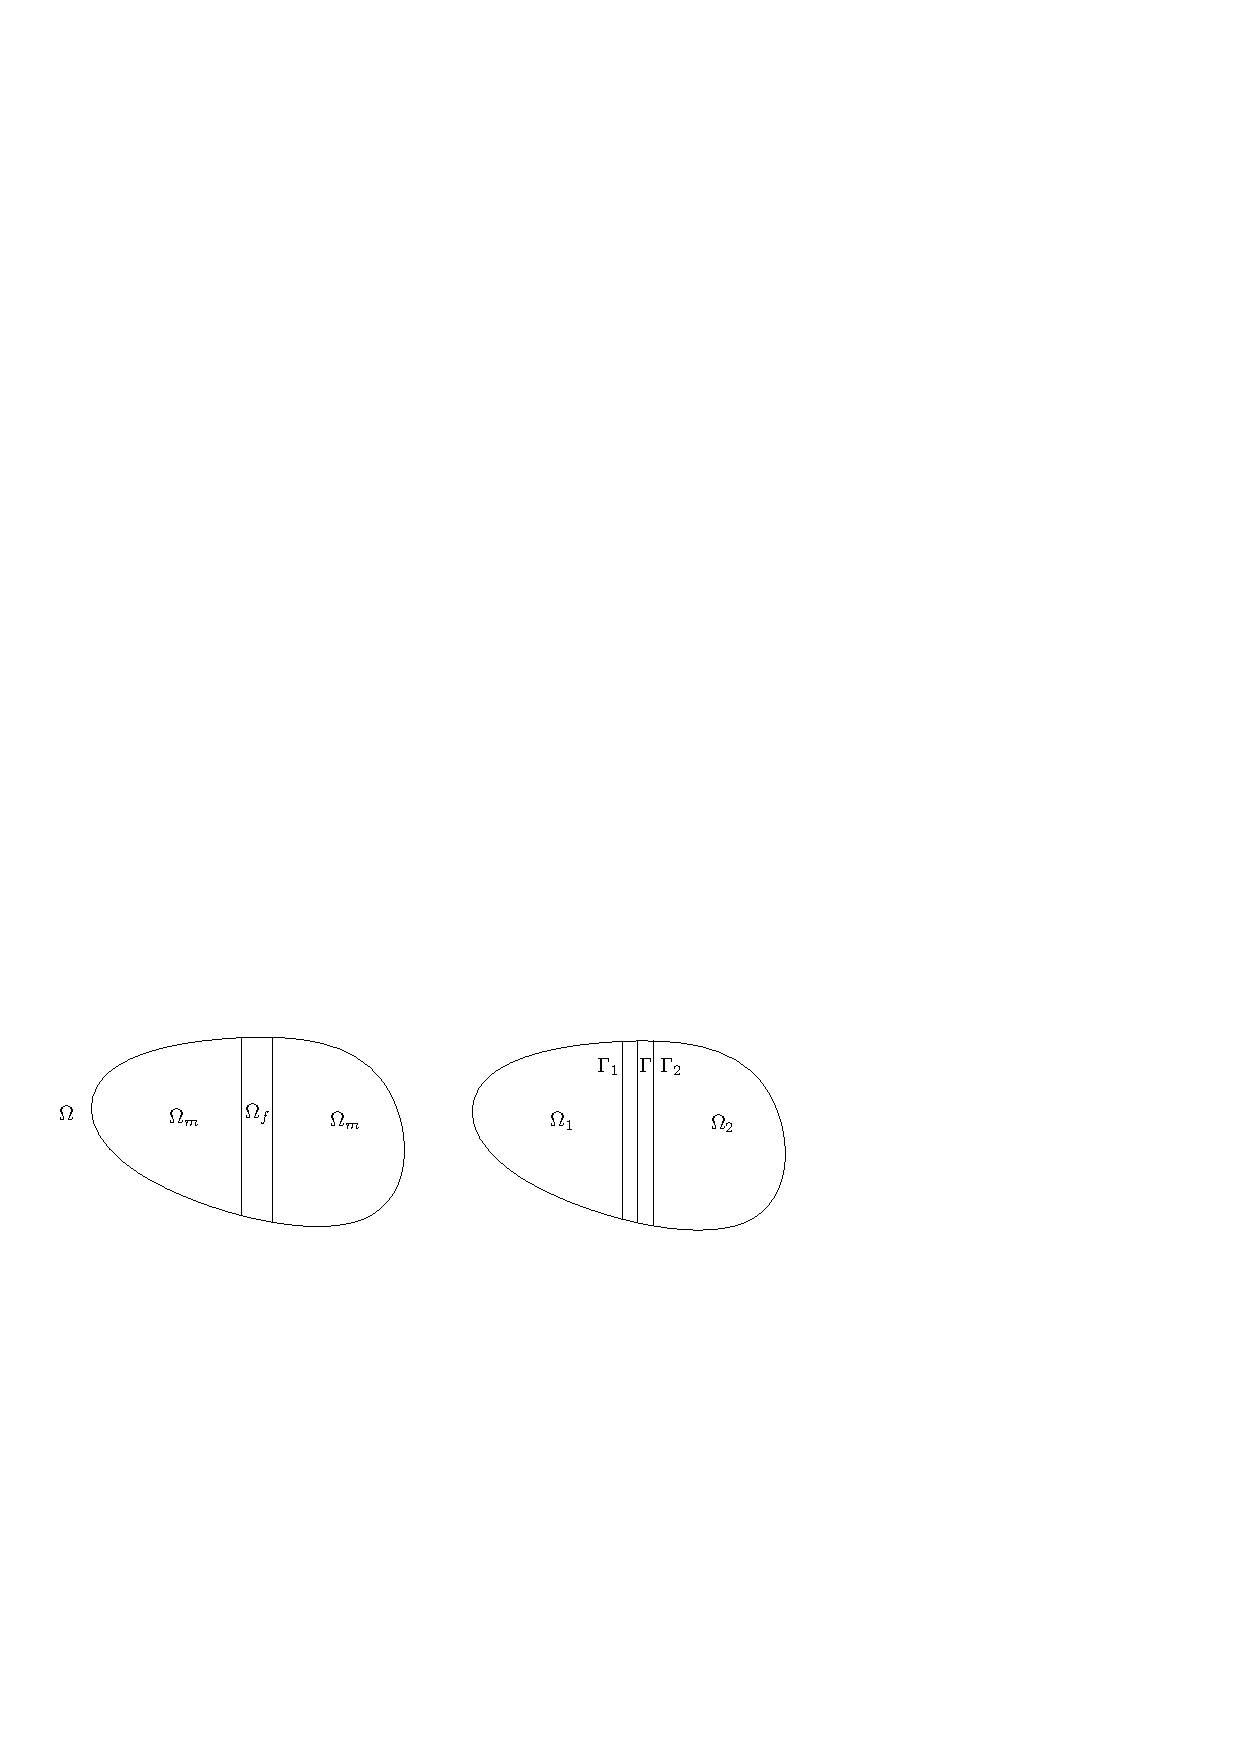
\includegraphics[width=12cm]{figures/domains}
\end{figure}

Fracture $\Omega_f\subset[-\delta/2,\delta/2]\times\Real^{d-1}$, $\Gamma:=(\{0\}\times\Real^{d-1})\cap\Omega_f$, $\Gamma_1:=(\{-\delta/2\}\times\Real^{d-1})\cap\Omega_f$, $\Gamma:=(\{\delta/2\}\times\Real^{d-1})\cap\Omega_f$

Domain $\Omega:=\Omega_1\cup\Gamma_1\cup\Omega_f\cup\Gamma_2\cup\Omega_2$, $\Omega_m:=\Omega_1\cup\Omega_2$ all Lipschitz domains

$\bar u(\vc y) := \frac1\delta\int_{-\delta/2}^{\delta/2}u(x,\vc y)\,dx$
(note: $u\in H^1(\Omega_f)\Rightarrow\bar u\in H^1(\Gamma)$)

Assumption: $\tn A_{|\Omega_f} = \begin{pmatrix}a_n&0\\0&\tn A_\tau\end{pmatrix}$, $\tn A_{|\Omega_f}=\tn A(\vc y)$

\paragraph{Global model.}
\[
-\div(\tn A\nabla u) = f \mbox{ in }\Omega,\qquad
u=0\mbox{ on }\partial\Omega
\]
Weak formulation: Find $u\in H^1_0(\Omega)$ such that for every $v\in H^1_0(\Omega)$:
\begin{equation}
\label{eq:weak_global}
\int_\Omega \tn A\nabla u\cdot\nabla v = \int_\Omega fv.
\end{equation}

\paragraph{Asymptotic model.}
\begin{align*}
-\div(\tn A\nabla u_m) &= f &&\mbox{ in }\Omega_m,\\
u_m &= 0 &&\mbox{ on }\partial\Omega\cap\partial\Omega_m,\\
-\tn A\nabla u_m\cdot\vc n &= Q(u_m,u_f) &&\mbox{ on }\Gamma_i,i=1,2,\\
-\div_\tau(\tn A_\tau\nabla_\tau u_f) &= \bar f + \frac1\delta\sum_{i=1}^2 Q(u_{m|\Gamma_i},u_f) &&\mbox{ in }\Gamma,\\
u_f &= 0 &&\mbox{ on }\Gamma\cap\partial\Omega,
\end{align*}
where $Q(w,z):=\frac2\delta a_n(w-z)$.

Weak formulation: Find $(u_m,u_f)\in H^1_{bc}(\Omega_m)\times H^1_0(\Gamma)$ such that:
\begin{subequations}
\label{eq:weak_asym}
\begin{equation}
\int_{\Omega_m}\tn A\nabla u_m\cdot\nabla v + \sum_{i=1}^2\int_\Gamma Q(u_{m|\Gamma_i},u_f)v_{|\Gamma_i} = \int_{\Omega_m} fv,
\end{equation}
\begin{equation}
\int_{\Gamma}\tn A_\tau\nabla_\tau u_f\cdot\nabla_\tau v = \int_\Gamma\bar f v + \frac1\delta\sum_{i=1}^2\int_\Gamma Q(u_{m|\Gamma_i},u_f)v.
\end{equation}
\end{subequations}


\begin{theorem}
Let $\tn A$ be uniformly bounded and positive definite in $\overline\Omega$, $f\in L^2(\Omega)$ and assume that the unique solution to \eqref{eq:weak_global} satisfies additionally $\partial_n^2 u\in C(\overline\Omega_f)$.
Then there is a constant $C:=C(\Omega,\Gamma,\tn A,\norm{\partial_n^2 u}_{\infty,\Omega_f},)>0$ such that
\begin{subequations}
\label{eq:error_estimates_delta}
\begin{align}
&\norm{\nabla_\tau(\bar u- u_f)}_{2,\Gamma} \le C\delta,\\
&\norm{\nabla(u-u_m)}_{2,\Omega_m} \le C\delta^{3/2},\\
&\sum_{i=1}^2\norm{\bar u-u_{|\Gamma_i}+u_{m|\Gamma_i}-u_f}_{2,\Gamma} \le C\delta^2.
\end{align}
\end{subequations}
\end{theorem}

\begin{proof}
Let us define for any $k\in\Natural$ an auxiliary operator $\Pi_k:L^2(\Omega_m)\times L^2(\Gamma)\to L^2(\Omega)$:
\begin{multline*}
\Pi_k(v_m,v_\Gamma)(x,\vc y)\\ :=
\begin{cases}
v_m(x,\vc y) & \mbox{ in }\Omega_m,\\
v_\Gamma(0,\vc y) & \mbox{ in }\Omega_{fk}:=\{(\tilde x,\tilde{\vc y})\in\Omega;~-\frac\delta2+\frac1k<\tilde x<\frac\delta2-\frac1k\},\\
k(x+\frac\delta2)v_\Gamma(0,\vc y) - k(x+\frac\delta2-\frac1k)v_m(-\frac\delta2,\vc y) & \mbox{ in }\{(\tilde x,\tilde{\vc y})\in\Omega;~\tilde x<-\frac\delta2+\frac1k\},\\
-k(x-\frac\delta2)v_\Gamma(0,\vc y) + k(x-\frac\delta2+\frac1k)v_m(\frac\delta2,\vc y) & \mbox{ in }\{(\tilde x,\tilde{\vc y})\in\Omega;~\tilde x>\frac\delta2-\frac1k\}.
\end{cases}
\end{multline*}
Note that $\Pi_k$ maps $H^1(\Omega_m)\times H^{1/2}(\Gamma)$ into $H^1(\Omega)$.
Hence we can test \eqref{eq:weak_global} by $v_k:=\Pi_k(u-u_m,\bar u-u_f)$, where $u$, $u_m$ and $u_f$ satisfy \eqref{eq:weak_global} and \eqref{eq:weak_asym}, respectively:
\begin{multline}
\label{eq:global_vk}
\int_{\Omega_m}\tn A\nabla u\cdot\nabla(u-u_m)
+\int_{\Omega_{fk}}\tn A_\tau\nabla_\tau u\cdot\nabla_\tau(\bar u-u_f)
+\int_{\Omega_f\setminus\Omega_{fk}} a_n\partial_n u \partial_n v_k\\
+ \int_{\Omega_f\setminus\Omega_{fk}} \tn A_\tau\nabla_\tau u \cdot \Pi_k(u-u_m,\nabla_\tau(\bar u-u_f))
= \int_{\Omega_m} f (u-u_m)\\
+ \int_{\Omega_{fk}} f (\bar u-u_f)
+ \int_{\Omega_f\setminus\Omega_{fk}} f v_k.
\end{multline}
Next we shall perform the limit $k\to\infty$.
Due to continuity of integral we have:
\begin{align}
&\int_{\Omega_{fk}}\tn A_\tau\nabla_\tau u\cdot\nabla_\tau(\bar u-u_f) \to \int_{\Omega_f}\tn A_\tau\nabla_\tau u\cdot\nabla_\tau(\bar u-u_f)\\
&\hspace{4cm} = \delta\int_\Gamma\tn A_\tau\nabla_\tau\bar u\cdot\nabla_\tau(\bar u-u_f),\\
&\int_{\Omega_f\setminus\Omega_{fk}} \tn A_\tau\nabla_\tau u \cdot \Pi_k(u-u_m,\nabla_\tau(\bar u-u_f)) \to 0, \\
&\int_{\Omega_{fk}} f (\bar u-u_f) \to \int_{\Omega_{f}} f (\bar u-u_f) = \delta\int_{\Gamma} \bar f (\bar u-u_f), \\
&\int_{\Omega_f\setminus\Omega_{fk}} f v_k \to 0,~k\to\infty.
\end{align}
The remaining term can be rewritten as follows:
\begin{multline}
\int_{\Omega_f\setminus\Omega_{fk}} a_n\partial_n u \partial_n v_k
= k\int_{-\frac\delta2}^{-\frac\delta2+\frac1k}\int_\Gamma a_n\partial_n u (\bar u - u_f - u_{|\Gamma_1} + u_{m|\Gamma_1})\\
+ k\int_{\frac\delta2-\frac1k}^{\frac\delta2}\int_\Gamma a_n\partial_n u (\bar u - u_f - u_{|\Gamma_2} + u_{m|\Gamma_2})\\
\to \sum_{i=1}^2\int_\Gamma a_n \partial_n u_{|\Gamma_i} (\bar u - u_f - u_{|\Gamma_i} + u_{m|\Gamma_i}),~k\to\infty.
\end{multline}
Since $\partial_n u$ is smooth, Taylor's expansion yields
\[ \partial_n u(\pm\frac\delta2,\vc y) = \frac2\delta(\bar u - u(\pm\frac\delta2,\vc y)) - \frac\delta3\partial_n^2 u(\xi(\vc y)),~\xi\in(-\frac\delta2,\frac\delta2), \]
i.e. there exist continuous functions $g_i\in C(\overline\Gamma)$ (independent of $\delta$) such that
\begin{equation}
\label{eq:taylor_for_du}
\partial_n u_{|\Gamma_i} = \frac2\delta(\bar u - u_{|\Gamma_i}) - \delta g_i,~i=1,2.
\end{equation}
Summing up, \eqref{eq:global_vk}--\eqref{eq:taylor_for_du} yield:
\begin{multline}
\label{eq:sum_global_vk_limit}
\int_{\Omega_m}\tn A\nabla u\cdot\nabla(u-u_m)
+\delta\int_\Gamma\tn A_\tau\nabla_\tau\bar u\cdot\nabla_\tau(\bar u-u_f)\\
+ \sum_{i=1}^2\int_\Gamma Q(\bar u,u_{|\Gamma_i}) (\bar u - u_{|\Gamma_i} + u_{m|\Gamma_i} - u_f)\\
= \int_{\Omega_m} f (u-u_m)
+ \delta\int_{\Gamma} \bar f (\bar u-u_f)
+ \delta\sum_{i=1}^2\int_\Gamma a_n g_i\, (\bar u - u_{|\Gamma_i} + u_{m|\Gamma_i} - u_f).
\end{multline}

Now we plug into \eqref{eq:weak_asym} test functions $u-u_m$, $\delta(\bar u-u_f)$, respectively, and add the resulting equations.
We obtain:
\begin{multline*}
\int_{\Omega_m}\tn A\nabla u_m\cdot\nabla(u-u_m) + \delta\int_\Gamma\tn A_\tau\nabla_\tau u_f\cdot\nabla_\tau(\bar u-u_f)\\
- \sum_{i=1}^2\int_\Gamma Q(u_{m|\Gamma_i},u_f)(\bar u - u_{|\Gamma_i}+u_{m|\Gamma_i} - u_f)
= \int_{\Omega_m} f(u-u_m)
+ \delta\int_\Gamma\bar f(\bar u-u_f).
\end{multline*}
Subtracting this from \eqref{eq:sum_global_vk_limit}, using H\"older's and Young's inequality yields:
\begin{multline}
\int_{\Omega_m}\tn A\nabla (u-u_m)\cdot\nabla(u-u_m)
+\delta\int_\Gamma\tn A_\tau\nabla_\tau(\bar u-u_f)\cdot\nabla_\tau(\bar u-u_f)\\
+ \sum_{i=1}^2\int_\Gamma \frac{2a_n}\delta |\bar u - u_{|\Gamma_i} + u_{m|\Gamma_i} - u_f|^2
= \delta\sum_{i=1}^2\int_\Gamma a_n g_i\, (\bar u - u_{|\Gamma_i} + u_{m|\Gamma_i} - u_f)\\
\le \left(\frac\delta2\right)^{\frac32}\sum_{i=1}^2\norm{\sqrt{a_n}g_i}_{\infty,\Gamma}\int_\Gamma\sqrt{\frac{2a_n}\delta}|\bar u - u_{|\Gamma_i} + u_{m|\Gamma_i} - u_f|\\
\le \frac{\delta^3}2\sum_{i=1}^2\norm{\sqrt{a_n}g_i}_{\infty,\Gamma} + \frac12\sum_{i=1}^2\int_\Gamma \frac{2a_n}\delta |\bar u - u_{|\Gamma_i} + u_{m|\Gamma_i} - u_f|^2.
\end{multline}
Finally we absorb the last term in the left hand side and use uniform positive definiteness of $\tn A$:
\begin{multline}
\norm{\nabla (u-u_m)}_{2,\Omega_m}^2
+\delta\norm{\nabla_\tau(\bar u-u_f)}_{2,\Gamma}^2\\
+ \frac1\delta\sum_{i=1}^2\norm{\bar u - u_{|\Gamma_i} + u_{m|\Gamma_i} - u_f}_{2,\Gamma}^2
\le C\delta^3,
\end{multline}
from which the estimates \eqref{eq:error_estimates_delta} follow.
\end{proof}




\subsection{Darcy flow model}
We consider simplest model for the velocity of the steady or unsteady flow in porous and fractured medium given by 
Darcy flow:
\begin{equation}
    \label{eq:darcy}
    \vc w = -\tn K \grad H \quad\text{on }\Omega_d,\ \text{for $d=1,2,3$}.
\end{equation}
We drop the dimension index of quantities in equations if it is the same as the dimension of the set where the equation holds.
In \eqref{eq:darcy}, $\vc w_d$ \units{}{1}{-1} is the superficial velocity,
$\tn K_d$ is the conductivity tensor, and $H_d$ \units{}{1}{} is the piezometric head. The velocity is related to the flux $\vc q_d$ 
with units \units{}{4-d}{-1} through
\[
    \vc q_d = \delta_d \vc w_d.
\]
where 
$\delta_d$ 
\units{}{3-d}{} is a cross section coefficient, in particular $\delta_3=1$, $\delta_2$ \units{}{1}{} is the thickness of a fracture, and $\delta_1$ \units{}{2}{} is the cross-section of a channel.
The flux $q_d$ is the volume of the liquid (water) that pass through a unit square ($d=3$),
unit line ($d=2$), or through a point ($d=1$) per one second. 
The conductivity tensor is given by the product \penalty-500
$\tn K_d = k_d \tn A_d$, where 
$k_d>0$ is the hydraulic conductivity \units{}{1}{-1} and 
$\tn A_d$ is 
$3\times 3$ dimensionless anisotropy tensor which has to be symmetric and positive definite. The piezometric-head $H_d$ is related to the pressure head
$h_d$ by $H_d = h_d + z$ assuming that the gravity force acts in negative direction of the $z$-axes. 
Combining these relations we get the Darcy law in the form:
\begin{equation}
    \label{eq:darcy_flux}
    \vc q = -\delta k\tn A \grad (h+z)  \qquad\text{on }\Omega_d,\ \text{for $d=1,2,3$}.
\end{equation}

Next, we employ continuity equation for saturated porous medium and the dimensional reduction from the preceding section (with $w=u:=H$, $\vc j:=\vc w$, $\tn A:=\tn K$ and $\vc b:=\vc 0$), which yields:
\begin{equation}
    \label{eq:continuity}
    \prtl_t (\delta S\, h) + \div \vc q = F \qquad \text{on }\Omega_d,\ \text{for $d=1,2,3$},
\end{equation}
where $S_d$ \units{}{-1}{} is the storativity and $F_d$ \units{}{3-d}{-1} is a source term. In our setting the principal unknowns of the system 
(\ref{eq:darcy_flux}, \ref{eq:continuity}) are the pressure head $h_d$ and the flux $\vc q_d$.


The storativity $S_d>0$ or the volumetric specific storage can be expressed as
\begin{equation}
  S_d = \gamma_w(\beta_r + \nu \beta_w),
\end{equation}
where $\gamma_w$ \units{1}{-2}{-2} is the specific weight of water, $\nu$ is the porosity $[-]$, $\beta_r$ is compressibility of the bulk material of the pores (rock)
and $\beta_w$ is compressibility of the water both with units \units{-1}{1}{-2}. For steady problems we set $S_d=0$ for all dimensions $d=1,2,3$.
The source term $F_d$ on the right hand side of \eqref{eq:continuity} consists of the volume density of prescribed sources 
$f_d$ \units{}{}{-1} and flux from higher dimension. 
Exact formula is slightly different for every dimension and will be discussed presently.

On $\Omega_3$ we simply have $F_3  = f_3$ \units{}{}{-1}.

On the set $\Omega_2 \cap \Omega_3$ the fracture is surrounded by one 3D surface from every side (or just one surface since we allow also 2D models on the boundary).
On $\prtl\Omega_3 \cap \Omega_2$ we prescribe boundary condition of Robin type
\begin{align*}
        \vc{q}_3\cdot \vc n^{+} &= q_{32}^{+} =\sigma_{3} (h_3^{+}-h_2),\\
        \vc{q}_3\cdot \vc n^{-} &= q_{32}^{-} =\sigma_{3} (h_3^{-}-h_2),
\end{align*}
where $\vc{q}_3\cdot\vc n^{+/-}$ \units{}{1}{-1} is the outflow from $\Omega_3$, $h_3^{+/-}$ is
a trace of the pressure head on $\Omega_3$, $h_2$ is the pressure head on $\Omega_2$, and 
$\sigma_{3}$ \units{}{}{-1} is the transition coefficient given by (see section \ref{sc:ad_on_fractures} and \cite{martin_modeling_2005})
\[
\label{e:sigma3_law}
  \sigma_3 = \sigma_{32} \frac{2\tn K_2 :\vc n_2\otimes\vc n_2 }{\delta_2}.
\]
Here $\vc n_2$ is the unit normal to the fracture (sign doesn't matter).
On the other hand, the sum of the interchange fluxes $q_{32}^{+/-}$ forms
a volume source on $\Omega_2$.  Therefore $F_2$ \units{}{1}{-1} on the right hand side of \eqref{eq:continuity} is
given by
\begin{equation}
   \label{source_2D}
   F_2 = \delta_2 f_2 + (q_{32}^{+} + q_{32}^{-}).
\end{equation}

The communication between $\Omega_2$  and  $\Omega_1$ is similar.  However, in the 3D ambient space,
an 1D channel can join multiple 2D fractures $1,\dots, n$. Therefore, we have $n$
independent outflows from $\Omega_2$:
\begin{equation*}
        \vc{q}_2\cdot \vc n^{i} = q_{21}^{i} =\sigma_{2} (h_2^{i}-h_1),
\end{equation*}
where $\sigma_2$ \units{}{1}{-1} is the transition coefficient integrated over the width of the fracture $i$:
\[
\label{e:sigma2_law}
  \sigma_2 = \sigma_{21} \frac{2\delta_2^2\tn K_1:{\vc n_1^i}\otimes{\vc n_1^i}}{\delta_1}.
\]
Here $\vc n_1^i$ is the unit normal to the channel that is tangential to the fracture $i$.
Sum of the fluxes forms part of $F_1$ \units{}{2}{-1}
\begin{equation}
   \label{source_1D}
   F_1 = \delta_1 f_1 + \sum_{i=1}^n q_{21}^{i}. 
\end{equation}
We remark that the direct communication between 3D and 1D is neglected.
The transition coefficients 
$\sigma_{32}$ \units{}{}{} and
$\sigma_{21}$ \units{}{}{} are independent scaling parameters which represent the ratio of the crosswind and the tangential conductivity in the fracture.

In order to obtain unique solution we have to prescribe boundary conditions. Currently we support three basic 
types of boundary condition. 
Consider disjoint decomposition of the boundary
\[
    \prtl\Omega_d = \Gamma_d^D \cap \Gamma_d^N \cap \Gamma_d^R
\]
into Dirichlet, Neumann, and Robin parts. We prescribe
\begin{align}
    h_d &= h_d^D        &&\text{ on }\Gamma_d^D,\\
    \vc q_d \cdot \vc n &= q_d^N         &&\text{ on }\Gamma_d^N,\\
    \vc q_d \cdot \vc n &= \sigma_d^R ( h_d - h_d^R)     &&\text{ on }\Gamma_d^R.
\end{align}
where 
$h_d^D$, $h_d^R$ 
is the given pressure head \units{}{1}{}, which alternatively can be prescribed through the piezometric head 
$H_d^D$, $H_d^R$ 
respectively. 
$q_d^N$ 
is the given surface density of the boundary outflow \units{}{4-d}{-1}, and  
$\sigma_d^R$ 
is the transition coefficient \units{}{3-d}{-1}.
The problem is well posed only if there is Dirichlet or Robin boundary condition on every component of the set $\Omega_1 \cup \Omega_2 \cup \Omega_3$ and $\sigma_d >0$ for 
$d=2,3$.

For unsteady problems one has to specify initial condition in terms of initial pressure head 
$h_d^0$ 
or initial piezometric head 
$H_d^0$.


% ***************************************** SYMBOLS
\def\abs#1{\lvert#1\rvert}
\def\argdot{{\hspace{0.18em}\cdot\hspace{0.18em}}}
\def\avg#1{\left\{#1\right\}_\omega}
\def\D{{\tn D}}
\def\div{\operatorname{div}}
\def\Eh{\mathcal E_h}       % edges of \Th
\def\Ehcom{\mathcal E_{h,C}}         % edges of \Th on interface with lower dimension
\def\Ehdir{\mathcal E_{h,D}}         % Dirichlet edges of \Th
\def\Ehint{\mathcal E_{h,I}}       % interior edges of \Th
\def\grad{\nabla}
\def\jmp#1{[#1]}
\def\n{\vc n}
\def\vc#1{\mathbf{\boldsymbol{#1}}}     % vector
\def\R{\mathbb R}
\def\sc#1#2{\left(#1,#2\right)}
\def\Th{\mathcal T_h}       % triangulation
\def\th{\vartheta}
\def\tn#1{{\mathbb{#1}}}    % tensor
\def\Tr{\operatorname{Tr}}
\def\where{\,|\,}
%***************************************************************************


\subsection{Transport of substances}
\label{sc:transport_model}

The motion of substances dissolved in water is governed by the \emph{advection}, and the \emph{hydrodynamic dispersion}.
In $\Omega_d$, $d\in\{1,2,3\}$, we consider the following system of mass balance equations\footnote{For $d\in\{1,2\}$ this form can be derived as in Section \ref{sc:ad_on_fractures} using $w:=\delta\th c^i$, $u:=c^i$, $\tn A:=\delta\th\tn D^i$, $\vc b:=\vc v=\frac{\vc q}{\th\delta}$.}:
\begin{equation}
    \label{e:ADE}
   \partial_t ( \delta \th c^i) + \div ( \vc q c^i ) - \div (\th \delta \D^i \grad c^i ) = F_S^i + F^c_C(c^i) + F_R(c^1,\dots, c^s).
\end{equation}
The principal unknown is the concentration $c^i$ \units{1}{-3}{} of a substance $i\in\{1,\dots, s\}$, which means weight of the substance in unit volume of the water.
Other quantities are:
\begin{itemize}

\item $\th$ \units{}{}{} is the porosity, i.e. fraction of space occupied by water and the total volume.
\item The hydrodynamic dispersivity tensor $\D^i$ \units{}{2}{-1} has the form
\begin{equation} 
  \label{eqn:transport_disp}
  \D^i =D_m^i \tau \tn I + \abs{\vc v}\left(\alpha_T^i \tn I + (\alpha_L^i - \alpha_T^i) \frac{\vc v \otimes \vc v}{\abs{\vc v}^2}\right),
\end{equation}
which represents (isotropic) molecular diffusion, and mechanical dispersion in longitudal and transversal direction to the flow.
Here $D_m^i$ \units{}{2}{-1} is the molecular diffusion coefficient of the $i$-th substance (usual magnitude in clear water is $10^{-9}$), $\tau=\th^{1/3}$ is the tortuosity (by \cite{millington_quirk}), $\alpha_L^i$ \units{}{1}{} and $\alpha_T^i$ \units{}{1}{} is the longitudal dispersivity and the transverse dispersivity, respectively.
Note that although we allow dispersivities to have different values for different substances, it is often assumed that they are intrinsic parameters of the porous medium.
Finally, $\vc v$ \units{}{1}{-1} is the \emph{microscopic} water velocity, related to the Darcy flux $\vc q$ by the relation $\vc q = \th\delta\vc v$.
The value of $D_m^i$ for specific substances can be found in literature (see e.g. \cite{cislerova_vogel}).
For instructions on how to determine $\alpha_L^i$, $\alpha_T^i$ we refer to \cite{marsily,domenico_schwartz}.

\item $F_S^i$ \units{1}{-d}{-1} represents the density of concentration sources.
Its form is:
\begin{equation}
 F_S^i = \delta f^i_S + \delta(c_S^i-c^i)\sigma_S. \label{eqn:transport_sources}
\end{equation}
Here $f_S^i$ \units{1}{-3}{-1} is the density of concentration sources, $c_S^i$ \units{1}{-3}{} is an equilibrium concentration and $\sigma_S^i$ \units{}{}{-1} is the concentration flux.

\item $F^c_C(c^i)$ \units{1}{-d}{-1} is the density of concentration sources due to exchange between regions with different dimensions, see \eqref{e:FC} below.

\item The reaction term $F_R(\dots)$ \units{1}{-d}{-1} is thoroughly described in the next section \ref{sec:reaction_term}.
\end{itemize}



\paragraph{Initial and boundary conditions.}
At time $t=0$ the concentration is determined by the initial condition
$$ c^i(0,\vc x) = c^i_0(\vc x). $$
The physical boundary $\partial\Omega_d$ is decomposed into the parts $\Gamma_I\cup\Gamma_D\cup\Gamma_N\cup\Gamma_R$, which may change during simulation time.
The first part $\Gamma_I$ is further divided into two segments:
\begin{align*}
\Gamma_I^+(t) &= \{\vc x\in \partial\Omega_d\where \vc q(t,\vc x)\cdot\vc n(\vc x)<0\},\\
\Gamma_I^-(t) &= \{\vc x\in \partial\Omega_d\where \vc q(t,\vc x)\cdot\vc n(\vc x)\ge 0\},
\end{align*}
where $\vc n$ stands for the unit outward normal vector to $\partial\Omega_d$.
We prescribe the following boundary conditions:
On the inflow parts $\Gamma_I^+\cup\Gamma_D$, the user must provide Dirichlet boundary condition $c_D^i$ for concentrations:
$$ c^i = c^i_D \mbox{ on }\Gamma_I^+\cup\Gamma_D. $$
On $\Gamma_I^-$ we impose homogeneous Neumann boundary condition:
$$ -\th\delta\D^i\nabla c^i\cdot\vc n = 0 \mbox{ on }\Gamma_I^-, $$
on $\Gamma_N$ we impose Neumann boundary condition with user-defined concentration flux $f^i_N$:
$$ -\th\delta\D^i\nabla c^i\cdot\vc n = f^i_N \mbox{ on }\Gamma_N, $$
and finally on $\Gamma_R$ we impose Robin boundary condition through transition parameter $\sigma^i_R$ and reference concentration $c^i_D$:
$$ -\th\delta\D^i\nabla c^i\cdot\vc n = \sigma^i_R(c^i-c^i_D) \mbox{ on }\Gamma_R. $$






\paragraph{Communication between dimensions.}
Transport of substances is considered also on interfaces of physical domains with adjacent dimensions (i.e. 3D-2D and 2D-1D, but not 3D-1D).
Denoting $c_{d+1}$, $c_d$ the concentration of a given substance in $\Omega_{d+1}$ and $\Omega_d$, respectively, the comunication on the interface between $\Omega_{d+1}$ and $\Omega_d$ is described by the quantity
\begin{equation}
  \label{e:inter_dim_flux}
  q^c_{d+1,d} = \sigma^c_{d+1,d} \frac{\delta_{d+1}^2}{\delta_d}2\th_d\D_d:\n\otimes\n ( c_{d+1} - c_d) + \begin{cases}q^l_{d+1,d} c_{d+1} & \mbox{ if }q^l_{d+1,d}\ge 0,\\q^l_{d+1,d} \frac{\th_d}{\th_{d+1}} c_d & \mbox{ if }q^l_{d+1,d}<0,\end{cases}
\end{equation}
where
\begin{itemize}
\item $q^c_{d+1,d}$ \units{1}{-d}{-1} is the density of concentration flux from $\Omega_{d+1}$ to $\Omega_d$,
\item $\sigma^c_{d+1,d}$ \units{}{}{} is a transition parameter.
Its value determines the mass exchange between dimensions whenever the concentrations differ.
In general, it is recommended to leave the default value $\sigma^c=1$ or to set $\sigma^c=0$ (when exchange is due to water flux only).
\item $q^l_{d+1,d}$ \units{}{3-d}{-1} is the water flux from $\Omega_{d+1}$ to $\Omega_d$, i.e. $q^l_{d+1,d} = \vc q_{d+1}\cdot\n_{d+1}$.
\end{itemize}
The communication between dimensions is incorporated as the total flux boundary condition for the problem on $\Omega_{d+1}$:
\begin{equation}
\label{e:FC}
-\th\delta\D\nabla c\cdot\vc n + q^w c = q^c
\end{equation}
and a source term in $\Omega_d$:
\begin{equation}
F^c_{C3} = 0,\quad
F^c_{C2} = q^c_{32},\quad
F^c_{C1} = q^c_{21}.
\end{equation}



\paragraph{Mass balance.}
The advection-dispersion equation satisfies the balance of mass in the following form:
$$ m^i(0) + \int_0^t s^i(\tau) \,d\tau - \int_0^t f^i(\tau) \,d\tau = m^i(t) $$
for any instant $t$ in the computational time interval and any substance $i$.
Here
$$ m^i(t) := \sum_{d=1}^3\int_{\Omega^d}(\delta\th c^i)(t,\vc x)\,d\vc x, $$
$$ s^i(t) := \sum_{d=1}^3\int_{\Omega^d}F_S^i(t,\vc x)\,d\vc x, $$
$$ f^i(t) := \sum_{d=1}^3\int_{\partial\Omega^d}\left(\vc q c^i - \th\delta\D^i\nabla c^i\right)(t,\vc x)\cdot\vc n \,d\vc x $$
is the mass \units{1}{}{}, the volume source \units{1}{}{-1} and the mass flux \units{1}{}{-1} of $i$-th substance at time $t$, respectively.
The mass, flux and source on every geometrical region is calculated at each computational time step and the values together with the control sums are written to the file \texttt{mass\_balance.txt}.


\paragraph{Two transport models.}
Within the above presented model, Flow123d presents two possible approaches to solute transport.
\begin{itemize}
\item For modelling pure advection ($\tn D=0$) one can choose {\tt TransportOperatorSplitting} method, which represents an explicit in time finite volume solver. The solution process for one time step is faster, but the maximal time step is restricted. The resulting concentration is piecewise constant on mesh elements. This solver supports reaction term (involving simple chemical reactions, dual porosity and adsorption).
\item The full model including dispersion is solved by {\tt SoluteTransport\_DG}, an implicit in time discontinuous Galerkin solver. It has no restriction of the computational time step and the space approximation is piecewise polynomial, currently up to order 3. Reaction term is currently not implemented.
\end{itemize}





%\section{Heat transfer}

Under the assumption of thermal equilibrium between the solid and liquid phase, the energy balance equation has the form\footnote{For lower dimensions this form can be derived as in Section \ref{sc:ad_on_fractures} using $w:=\delta\tilde s T$, $u:=T$, $\tn A:=\delta\lambda\tn I$, $\vc b:=\frac{\varrho_l c_l}{\tilde s}\vc w$.}
\[
    \partial_t\left(\delta \tilde s T \right) + \div(\varrho_l c_l T \vc q) - \div(\delta\Lambda\nabla T) = F^T + F^T_C.
\]
The principal unknown is the temperature $T$ [K].
Other quantities are:
\begin{itemize}
\item \hyperA{HeatTransfer-DG-Data::fluid-density}{$\varrho_l$}, \hyperA{HeatTransfer-DG-Data::solid-density}{$\varrho_s$} \units{1}{-3}{} is the density of the fluid and solid phase, respectively.
\item \hyperA{HeatTransfer-DG-Data::fluid-heat-capacity}{$c_l$}, \hyperA{HeatTransfer-DG-Data::solid-heat-capacity}{$c_s$} [J$\mathrm{kg}^{-1}\mathrm{K}^{-1}$] is the heat capacity of fluid and solid phase, respectively.
\item $\tilde s$ [J$\mathrm{m}^{-3}\mathrm{K}^{-1}$] is the volumetric heat capacity of the porous medium defined as
\[ \tilde s = \hyperA{HeatTransfer-DG-Data::porosity}{\th}\varrho_l c_l + (1-\th)\varrho_s c_s. \]
\item $\Lambda$ [W$\mathrm{m}^{-1}\mathrm{K}^{-1}$] is the thermal dispersion tensor:
\[ \Lambda = \Lambda^{cond} + \Lambda^{disp} \]
\[ \Lambda^{cond} = \left(\th \lambda_l^{cond} + (1-\th)\lambda_s^{cond}\right)\tn I, \]
\[ \Lambda^{disp} = \th \varrho_l c_l|\vc v|\left(\alpha_T\tn I + (\alpha_L-\alpha_T)\frac{\vc v\otimes\vc v}{|\vc v|^2}\right), \]
where \hyperA{HeatTransfer-DG-Data::fluid-heat-conductivity}{$\lambda_l^{cond}$}, \hyperA{HeatTransfer-DG-Data::solid-heat-conductivity}{$\lambda_s^{cond}$} [W$\mathrm{m}^{-1}\mathrm{K}^{-1}$] is the thermal conductivity of the fluid and solid phase, respectively, and \hyperA{HeatTransfer-DG-Data::disp-l}{$\alpha_L$}, \hyperA{HeatTransfer-DG-Data::disp-t}{$\alpha_T$} \units{}{1}{} is the longitudal and transverse dispersivity in the fluid.

\item $F^T$ [J$\mathrm{m}^{-d}\mathrm{s}^{-1}$] represents the thermal source:
\[ F^T = \delta \th F^T_l + \delta (1-\th) F^T_s, \]
\[ F^T_l = f_l^T + \varrho_l c_l \sigma^T_l(T-T_l), \]
\[ F^T_s = f_s^T + \varrho_s c_s \sigma^T_s(T-T_s), \]
where \hyperA{HeatTransfer-DG-Data::fluid-thermal-source}{$f_l^T$}, \hyperA{HeatTransfer-DG-Data::solid-thermal-source}{$f_s^T$} [W$\mathrm{m}^{-3}$] is the density of thermal sources in fluid and solid, respectively, \hyperA{HeatTransfer-DG-Data::fluid-ref-temperature}{$T_l$}, \hyperA{HeatTransfer-DG-Data::solid-ref-temperature}{$T_s$} [K] is a reference temperature and \hyperA{HeatTransfer-DG-Data::fluid-heat-exchange-rate}{$\sigma^T_l$}, \hyperA{HeatTransfer-DG-Data::solid-heat-exchange-rate}{$\sigma^T_s$} \units{}{}{-1} is the heat exchange rate.
\end{itemize}



\paragraph{Initial and boundary conditions.}
At time $t=0$ the temperature is determined by the initial condition
$$ T(0,\vc x) = \hyperA{HeatTransfer-DG-Data::init-temperature}{T_0}(\vc x). $$
Given the decomposition of $\partial\Omega_d$ into $\Gamma_I\cup\Gamma_D\cup\Gamma_N\cup\Gamma_R$ (see Section \ref{sc:transport_model}), we prescribe the following boundary conditions:
\begin{itemize}
\item Dirichlet:
\[ T = \hyperA{HeatTransfer-DG-Data::bc-temperature}{T_D} \mbox{ on }\Gamma_I^+\cup\Gamma_D, \]
\item Homogeneous Neumann:
\[ \left(\varrho_l c_l T \vc q - \delta\Lambda\nabla T\right)\cdot\vc n = 0 \mbox{ on }\Gamma_I^-, \]
\item Neumann:
\[ \left(\varrho_l c_l T \vc q - \delta\Lambda\nabla T\right)\cdot\vc n = \hyperA{HeatTransfer-DG-Data::bc-flux}{f_N} \mbox{ on }\Gamma_N, \]
\item Robin (Newton):
\[ \left(\varrho_l c_l T \vc q - \delta\Lambda\nabla T\right)\cdot\vc n = \hyperA{HeatTransfer-DG-Data::bc-robin-sigma}{\sigma_R}(T-\hyperA{HeatTransfer-DG-Data::bc-temperature}{T_D}) \mbox{ on }\Gamma_R. \]
\end{itemize}






\paragraph{Communication between dimensions.}
Denoting $T_{d+1}$, $T_d$ the temperature in $\Omega_{d+1}$ and $\Omega_d$, respectively, the communication on the interface between $\Omega_{d+1}$ and $\Omega_d$ is described by the quantity
\begin{equation}
  \label{e:inter_dim_flux_heat}
  q^T_{d+1,d} = \sigma^T_{d+1,d} \frac{\delta_{d+1}^2}{\delta_d}2\Lambda_d:\n\otimes\n ( T_{d+1} - T_d) + \begin{cases} \varrho_l c_l q^l_{d+1,d} T_{d+1} & \mbox{ if }q^l_{d+1,d}\ge 0,\\\varrho_l c_l q^l_{d+1,d} \frac{\tilde s_d}{\tilde s_{d+1}} T_d & \mbox{ if } q^l_{d+1,d}<0,\end{cases}
\end{equation}
where
\begin{itemize}
\item $q^T_{d+1,d}$ [W$\mathrm{m}^{-2}$] is the density of heat flux from $\Omega_{d+1}$ to $\Omega_d$,
\item \hyperA{HeatTransfer-DG-Data::fracture-sigma}{$\sigma^T_{d+1,d}$} \units{}{}{} is a transition parameter.
Its value determines the exchange of energy between dimensions due to temperature difference.
In general, it is recommended to leave the default value $\sigma^T=1$ or to set $\sigma^T=0$ (when exchange is due to water flux only).
\item $q^l_{d+1,d}=\vc q_{d+1}\cdot\vc n$ is the water flux from $\Omega_{d+1}$ to $\Omega_d$.
\end{itemize}
The communication between dimensions is incorporated as the total flux boundary condition for the problem on $\Omega_{d+1}$:
\begin{equation}
\label{e:heat_FC}
\left(\varrho_l c_l T \vc q - \delta\Lambda\nabla T\right)\cdot\vc n = q^T
\end{equation}
and a source term in $\Omega_d$:
\begin{equation}
F^T_{C3} = 0,\quad
F^T_{C2} = q^T_{32},\quad
F^T_{C1} = q^T_{21}.
\end{equation}




\paragraph{Energy balance.}
The heat equation satisfies the balance of energy in the following form:
$$ e(0) + \int_0^t s(\tau) \,d\tau - \int_0^t f(\tau) \,d\tau = e(t) $$
for any instant $t$ in the computational time interval.
Here
$$ e(t) := \sum_{d=1}^3\int_{\Omega^d}(\delta \tilde s T)(t,\vc x)\,d\vc x, $$
$$ s(t) := \sum_{d=1}^3\int_{\Omega^d}F_S^T(t,\vc x)\,d\vc x, $$
$$ f(t) := \sum_{d=1}^3\int_{\partial\Omega^d}\left(\varrho_l c_l T\vc q - \delta\Lambda\nabla T\right)(t,\vc x)\cdot\vc n \,d\vc x $$
is the energy [J], the volume source [J$\mathrm{s}^{-1}$] and the energy flux [J$\mathrm{s}^{-1}$] at time $t$, respectively.
The energy, flux and source on every geometrical region is calculated at each computational time step and the values together with the control sums are written to the file \texttt{mass\_balance.txt}.









\bibliographystyle{abbrvnat}
\bibliography{flow123d_doc.bib}
%%%%%%%%%%%%%%%%%%%%%%%%%%%%%%%%%%%%%%%%%%%%%%%%%%%%%%%%%%%%%%%%%%%%%%%%%%%%%%%%%%%%%%%%%%%%%%%%%%%%%%%%%%%%%%%%%


\end{document}


